\chapter{Криптографические хэш-функции}\label{chapter-hash-functions}
\selectlanguage{russian}

Хэш-функции возникли как один из вариантов решения задачи <<поиска по словарю>>. Задача состояла в поиске в памяти компьютера (оперативной или постоянной) информации по известному ключу. Возможным способом решения было хранение, например, всего массива ключей (и указателей на содержимое) в отсортированном в некотором порядке списке, либо в виде бинарного дерева. Однако наиболее производительным с точки зрения времени доступа (при этом обладая допустимой производительностью по времени модификации) стал метод хранения в виде хэш-таблиц. Этот метод ведёт своё происхождение из стен компании IBM (как и многое другое в программировании).

Метод хэш-таблиц подробно разобран в любой современной литературе по программированию~\cite{Knuth:2001:3}. Напомним лишь, что его идея состоит в разделении множества ключей по корзинам (bins) в зависимости от значения некоторой функции, вычисляемой по значению ключа. Причём функция подбирается таким образом, чтобы в разных корзинах оказалось одинаковое число (в идеале -- не более одного) ключей. При этом сама функция должна быть быстро вычисляемой, а её значение должно легко конвертироваться в натуральное число, которое не превышает число корзин.

\emph{Хэш-функцией} (\langen{hash function}) называется отображение, переводящее аргумент произвольной длины в значение фиксированной длины.

\emph{Коллизией} хэш-функции называется пара значений аргумента, дающая одинаковый выход хэш-функции. Коллизии есть у любых хэш-функций, если количество различных значений аргумента превышает возможное количество значений результата функции (принцип Дирихле). А если не превышает, то и нет смысла использовать хэш-функцию.

\example
Приведём пример метода построения хэш-функции, называемого методом Меркла~---~Дамгарда\index{структура!Меркла~---~Дамгарда}~\cite{Merkle:1979, Merkle:1990, Damgard:1990}.

Пусть имеется файл $X$ в виде двоичной последовательности некоторой длины. Разделяем $X$ на несколько отрезков фиксированной длины, например по 256 символов:  $m_{1} ~\|~ m_{2} ~\|~ m_{3} ~\|~ \ldots ~\|~ m_{t}$. Если длина файла $X$ не является кратной 256 битам, то последний отрезок дополняем нулевыми символами и обозначаем $m'_{t}$.
Обозначим за $t$ новую длину последовательности. Считаем каждый отрезок $m_i, ~ i = 1, 2, \dots, t$ двоичным представлением целого числа.

Для построения хэш-функции используем рекуррентный способ вычисления. Предварительно введём вспомогательную функцию $\chi(m, H)$, называемую функцией компрессии или сжимающей функцией. Задаём начальное значение $H_{0} = 0^{256} \equiv \underbrace{000 \ldots 0}_{256} $. Далее вычисляем:
\[ \begin{array}{l}
    H_1 = \chi( m_1, H_0), \\
    H_2 = \chi( m_2, H_1), \\
    \dots,\\
    H_t = \chi( m'_t, H_{t-1}). \\
\end{array} \]
Считаем $H_{t} = h(X)$ хэш-функцией.
\exampleend

В программировании к свойствам хорошей хэш-функции относят:
\begin{itemize}
    \item быструю скорость работы;
    \item минимальное число коллизий.
\end{itemize}

Можно назвать и другие свойства, которые были бы полезны для хэш-функции в программировании. К ним можно отнести, например, отсутствие необходимости в дополнительной памяти (неиспользование <<кучи>>), простоту реализации, стабильность работы алгоритма (возврат одного и того же результата после перезапуска программы), соответствие результатов работы хэш-функции результатам работы других функций, например, функций сравнения (см. например, описания функций \texttt{hashcode()}, \texttt{equals()} и \texttt{compare()} в языке программирования Java).

\emph{Однонаправленной функцией}\index{функция!однонаправленная} $f(x)$ называется функция, обладающая следующими свойствами:
\begin{itemize}
    \item вычисление значения функции $f(x)$ для всех значений аргумента $x$ является \emph{вычислительно лёгкой} задачей;
    \item нахождение аргумента $x$, соответствующего значению функции $f(x)$, является \emph{вычислительно трудной} задачей.
\end{itemize}

Свойство однонаправленности, в частности, означает, что если в аргументе $x$ меняется хотя бы один символ, то для любого $x$ значение функции $H(x)$ меняется непредсказуемо.

\emph{Криптографической хэш-функцией} $H(x)$ называется хэш-функция, имеющая следующие свойства:
\begin{itemize}
    \item однонаправленность: \emph{вычислительно невозможно} по значению функции найти прообраз;
    \item \emph{слабая устойчивость к коллизиям}\index{устойчивость к коллизиям} (слабо бесконфликтная функция): для заданного аргумента $x$ \emph{вычислительно невозможно} найти другой аргумент $y \neq x: ~ H(x) = H(y)$;
    \item \emph{сильная устойчивость к коллизиям} (сильно бесконфликтная функция): \emph{вычислительно невозможно} найти пару разных аргументов $x \neq y: ~ H(x) = H(y)$.
\end{itemize}

Из требования на устойчивость к коллизиям, в частности, следует свойство (близости к) равномерности распределения хэш-значений.

При произвольной длине последовательности $X$ длина хэш-функции $H(X)$ в российском стандарте ГОСТ Р 34.11-94 равна 256-ти символам, в американском стандарте SHA несколько различных значений длин: 160, 192, 256, 512 символов.

\section{ГОСТ Р 34.11-94}\index{хэш-функция!ГОСТ Р 34.11-94|(}
\selectlanguage{russian}

Представим описание устаревшего российского стандарта хэш-функции ГОСТ Р 34.11-94~\cite{GOST-94}.

Пусть $X$ -- последовательность длины 256 бит. Запишем $X$ тремя способами в виде конкатенации блоков:
\[ \begin{array}{ll}
    X & = X_4 ~\|~ X_3 ~\|~ X_2 ~\|~ X_1 = \\
    & = ~ \eta_{16} ~\|~ \eta_{15} ~\|~ \dots ~\|~ \eta_2 ~\|~ \eta_1 = \\
    & = ~ \xi_{32} ~\|~ \xi_{31} ~\|~ \dots ~\|~ \xi_2 ~\|~ \xi_1
\end{array} \]
с длинами 64, 16 и 8 бит соответственно.

Введём три функции:
\[ \begin{array}{ll}
    A(X) & \equiv A(X_4 ~\|~ X_3 ~\|~ X_2 ~\|~ X_1) = \\
        & = \left( X_1 \oplus X_2 \right) ~\|~ X_4 ~\|~ X_3 ~\|~ X_2, \\
    & \\
    \psi(X) & \equiv \psi(\eta_{16} ~\|~ \eta_{15} ~\|~ \dots ~\|~ \eta_2 ~\|~ \eta_1) = \\
        & = \left( \eta_1 \oplus \eta_2 \oplus \dots \oplus \eta_{15} \right) ~\|~
            \eta_{16} ~\|~ \eta_{15} ~\|~ \dots ~\|~ \eta_3 ~\|~ \eta_2, \\
    & \\
    P(X) & \equiv P(\xi_{32} ~\|~ \xi_{31} ~\|~ \dots ~\|~ \xi_2 ~\|~ \xi_1) = \\
        & = \xi_{\varphi(32)} ~\|~ \xi_{\varphi(31)} ~\|~ \dots ~\|~ \xi_{\varphi(2)} ~\|~ \xi_{\varphi(1)},
\end{array} \]
где $\varphi(s)$ -- перестановка байта, $s$ -- номер байта. Функции $A(X)$ и $\psi(X)$ -- регистры сдвига с линейной обратной связью.

Число $s$ однозначно представляется через целые числа $i,k$, и правило перестановки $\varphi(s)$ записывается:
\[ \begin{array}{c}
    s = i + 4 (k - 1) + 1, ~~ 0 \leq i \leq 3, ~ 1 \leq k \leq 8, \\
    \varphi(s) = 8 i + k. \\
\end{array} \]
Приведём пример. Пусть $s = 7$, тогда $i=2, k=2$. Находим перестановку $\varphi(7) = 8 \cdot 2 + 2 = 18$. Седьмой байт переместился на 18-е место.

В российском стандарте функция компрессии двух 256-битовых блоков сообщения $M$ и результата хэширования предыдущего блока $H$ имеет вид
\[
    H' = \chi(M, H) = \psi^{61}(H \oplus \psi(M \oplus \psi^{12}(S))),
\]
где $\psi^j(X)$ -- суперпозиция $j$ функций $\psi( \psi( \dots ( \psi( X)) \dots ))$, ~ 256-битовый блок $S$ определяется ниже.

256-битовые блоки $H$ и $S$ представляются конкатенацией четырёх 64-битовых блоков
\[ \begin{array}{l}
    H = h_4 ~\|~ h_3 ~\|~ h_2 ~\|~ h_1, \\
    S = s_4 ~\|~ s_3 ~\|~ s_2 ~\|~ s_1, \\
    s_i = E_{K_i}( h_i), ~ i = 1, 2, 3, 4, \\
\end{array} \]
где $E_{K_i}( h_i)$ -- криптографическое преобразование 64-битового блока $h_i$ стандарта блочного шифрования ГОСТ 28147-89 с помощью ключа шифрования $K_i$.

Вычисление ключей $K_i$ производится через вспомогательные функции:
\[ \begin{array}{c}
    U_1 = H, ~~ V_1 = M, \\
    U_i = A(U_{i-1}) \oplus C_i, ~~ V_i = A(A(V_{i-1})), ~~ i = 2, 3, 4, \\
\end{array} \]
где $C_2, C_3, C_4$ -- 256-битовые блоки:
\[ \begin{array}{c}
    C_2 = C_4 = 0^{256}, \\
    C_3 = 1^8 0^8 1^{16} 0^{24} 1^{16} 0^8 (0^8 1^8)^2 1^8 0^8 (0^8 1^8)^4 (1^8 0^8)^4. \\
\end{array} \]
Окончательно получаем ключи
\[
    K_i = P(U_i \oplus V_i), ~ i = 1,2,3,4.
\]

%Ключевая хэш-функция определяется в виде $h_{K} (X)=h(KXK)$, где $h(X)$ -- некоторая стандартная хэш-функция, $K$ -- секретный ключ.
\index{хэш-функция!ГОСТ Р 34.11-94|)}


\section{Хэш-функция «Стрибог»}\label{section-stribog}\index{хэш-функция!«Стрибог»|(}
\selectlanguage{russian}

С 1 января 2013 года в России введён в действие новый стандарт на криптографическую хэш-функцию ГОСТ Р 34.11-2012~\cite{GOST-R:34.11-2012}. Неофициально новый алгоритм получил название <<Стрибог>>. При разработке хэш-функции авторы основывались на нескольких требованиях:

\begin{itemize}
	\item не должна быть уязвима к известным атакам;
	\item должна использовать хорошо изученные конструкции и преобразования;
	\item не должно быть лишних преобразований, каждое преобразование должно гарантировать выполнение определённых криптографических свойств;
	\item при наличии нескольких вариантов реализации требуемого свойства -- наиболее простой для анализа и реализации;
	\item максимальная производительность \emph{программной} реализации.
\end{itemize}

В соответствии с данными требованиями алгоритм новой хэш-функции основывается на хорошо изученных конструкциях Меркла~---~Дамгарда\index{структура!Меркла~---~Дамгарда}~\cite{Merkle:1979, Merkle:1990, Damgard:1990} и Миагучи~---~Пренеля\index{структура!Миагучи~---~Пренеля}~\cite{Espen:Mieghem:1989, Miyaguchi:Ohta:Iwata:1990:03, Miyaguchi:Ohta:Iwata:1990:11}, во внешней своей структуре практически полностью повторяя режим HAIFA\index{HAIFA} (\langen{HAsh Iterative FrAmework},~\cite{Biham:Dunkelman:2007}), использовавшийся в хэш-функциях SHAvite-3\index{хэш-функция|SHAvite-3} и BLAKE\index{хэш-функция|BLAKE}.

\begin{figure}[htb]
	\centering
	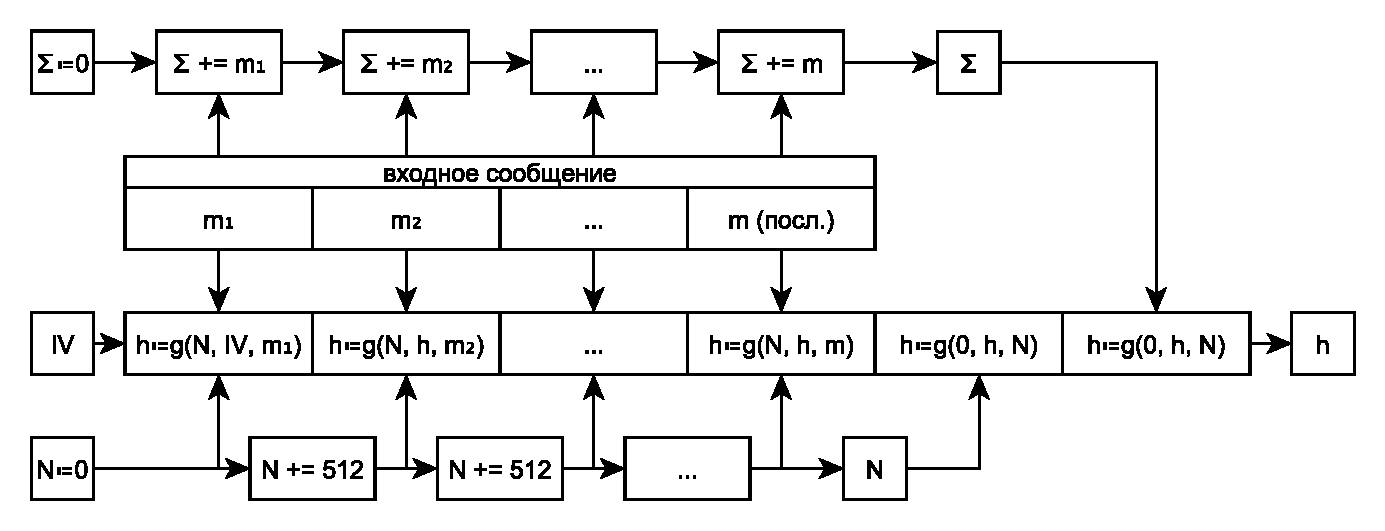
\includegraphics[width=0.95\textwidth]{pic/stribog-md}
  \caption{Использование структуры Меркла~---~Дамгарда в хэш-функции <<Стрибог>>}
  \label{fig:stribog-md}
\end{figure}

Как показано на рис.~\ref{fig:stribog-md}, входное сообщение разбивается на блоки по 512 бит (64 байта). Последний блок \emph{слева} дополняется последовательностью из нулей и  одной единицы до 512 бит (длина дополнения не учитывается в дальнейшем, когда длина сообщения используется как аргумент функций). Для каждой части сообщения вычисляется значение функции $g_N(h, m)$, которая в качестве аргумента использует текущий номер блока (умноженный на 512), результат вычисления для предыдущего блока и очередной блок сообщения. Также есть два завершающих преобразования. Первое вместо блока сообщения использует количество обработанных бит N (то есть длину сообщения), а второе -- арифметическую сумму значений всех блоков сообщения. В предположении, что функция $g_N(h, m)$ является надёжной для создания криптографически стойких хэш-функций, известно, что конструкция Меркла~---~Дамгарда позволяет получить хэш-функцию со следующими параметрами:

\begin{itemize}
	\item сложность построения прообраза: $2^n$ операций;
	\item сложность построения второго прообраза: $2^n / \left|M\right|$ операций;
	\item сложность построения коллизии: $2^{n/2}$ операций;
	\item сложность удлинения прообраза: $2^n$ операций.
\end{itemize}

Все параметры совпадают с аналогичными для идеальной хэш-функции, кроме сложности построения второго прообраза, который равен $2^n$ для идеального алгоритма.

В качестве функции $g_N(h, m)$ используется конструкция Миагучи~---~Пренеля\index{структура!Миагучи~---~Пренеля} (см. рис.~\ref{fig:stribog-mp}), которая является стойкой ко всем атакам, известным для схем однонаправленных хэш-функций на базе симметричных алгоритмов, в том числе к атаке с <<фиксированной точкой>>~\cite[стр. 502]{Schneier:2002}. \emph{Фиксированной точкой}\index{точка!фиксированная} называется пара чисел $(h, m)$, для которой у заданной функции $g$ выполняется $g(h, m) = h$.

\begin{figure}[htb]
	\centering
	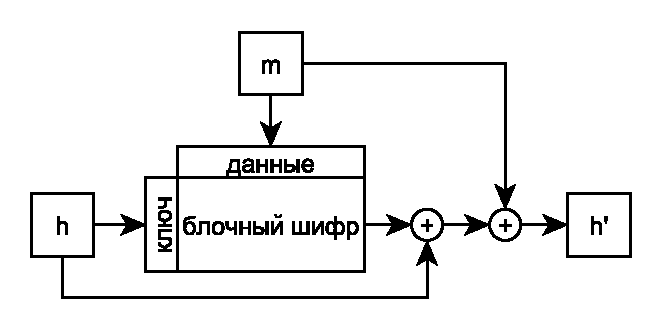
\includegraphics[width=0.66\textwidth]{pic/stribog-mp}
  \caption{Использование структуры Миагучи~---~Пренеля в хэш-функции <<Стрибог>>}
  \label{fig:stribog-mp}
\end{figure}

\index{шифр!XSPL|(}В качестве блочного шифра используется новый XSPL-шифр, изображённый на рис.~\ref{fig:stribog-xspl}, отдельные элементы и идеи которого позже войдут в новый стандарт <<Кузнечик>>\index{шифр!<<Кузнечик>>} (см. раздел~\ref{section-grig}). Шифр является примером шифра на основе SP-сети\index{SP-сеть} (сети замен и перестановок), каждый раунд которого является набором обратимых преобразований над входным блоком.

\begin{figure}[htb]
	\centering
	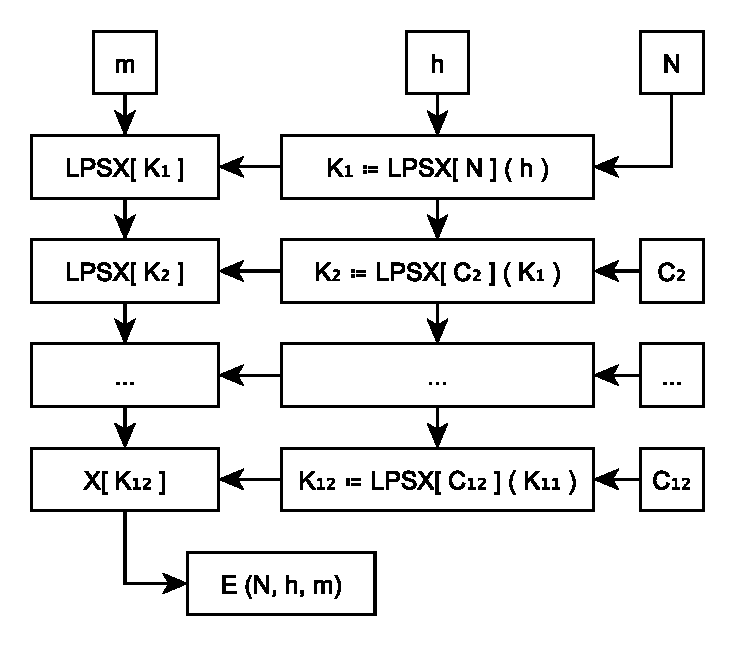
\includegraphics[width=0.75\textwidth]{pic/stribog-xspl}
  \caption{XSPL-шифр в хэш-функции <<Стрибог>>}
  \label{fig:stribog-xspl}
\end{figure}

Каждый раунд XSPL-шифра, кроме последнего, состоит из следующих обратимых преобразований:
\begin{itemize}
	\item $X\left[C\right]$ -- побитовое сложение по модулю 2 с дополнительным аргументом $C$;
	\item $S$ -- нелинейная обратимая замена байтов;
	\item $P$ -- перестановка байтов внутри блока данных (транспонирование матрицы размером $8 \times 8$ из ячеек по одному байту каждая);
	\item $L$ -- обратимое линейное преобразование (умножение векторов на фиксированную матрицу).
\end{itemize}

Особенностью предложенного шифра является полная аналогия между алгоритмом развёртывания ключа и алгоритмом, собственно, преобразования открытого текста. В качестве <<раундовых ключей>> для алгоритма развёртывания ключа на первом раунде используется общее число уже обработанных бит хэш-функцией N, а на остальных раундах -- 512-битные константы, заданные в стандарте.\index{шифр!XSPL|)}

Новый алгоритм, согласно отдельным исследованиям, до полутора раз быстрее предыдущего стандарта ГОСТ Р 34.11-94\index{хэш-функция!ГОСТ Р 34.11-94}, используя 27 тактов на один байт входного сообщения (94~МБ/с), против 40 для старого стандарта (64~МБ/с)\footnote{Реализации тестировались на процессоре Intel Core i7-920 CPU @ 2.67~GHz и видеокарте NVIDIA GTX 580. См.~\cite{Lebedev:2013}}.

В 2014 году группа исследователей (\cite{Guo:Jean:Leurent:Peyrin:Wang:2014}) обнаружила недостаток в реализации конструкции HAIFA в хэш-функции <<Стрибог>>, который ведёт к уменьшению сложности атаки по поиску второго прообраза до $n \times 2^{n/2}$, то есть до $2^{266}$. Авторы работы получили первую премии в размере пятьсот тысяч рублей на конкурсе по исследованию хэш-функции «Стрибог», проводившимся Российским Техническим комитетом по стандартизации «Криптографическая защита информации» (ТК~26) при участии Академии криптографии Российской Федерации и при организационной и финансовой поддержке ОАО «ИнфоТеКС».

\index{хэш-функция!«Стрибог»|)}


\section{Коды аутентификации сообщений}
\selectlanguage{russian}

Для обеспечения целостности и подтверждения авторства информации, передаваемой по каналу связи, используют \textbf{коды аутентификации сообщений}, $\MAC$ (message authentication code).

Кодом аутентификации сообщения называется \emph{криптографическая хэш-функция} $\MAC(K,m)$, зависящая от передаваемого сообщения $m$ и секретного ключа $K$ отправителя $A$, обладающая свойствами цифровой подписи:
\begin{itemize}
    \item получатель $B$, используя такой же или другой ключ, имеет возможность проверить целостность и доказать принадлежность информации $A$;
    \item код аутентификации невозможно фальсифицировать.
\end{itemize}

Код аутентификации может быть построен либо на симметричной криптосистеме, в таком случае обе стороны имеют один общий секретный ключ, либо на криптосистеме с открытым ключом, в которой $A$ использует свой секретный ключ, а $B$ -- открытый ключ отправителя $A$.

Наиболее универсальный способ аутентификации сообщений через схемы ЭП на криптосистемах с открытым ключом состоит в том, что сторона $A$ отправляет стороне $B$ сообщение
    \[ m ~\|~ \textrm{ЭП}(K, h(m)), \]
где $h(m)$ -- криптографическая хэш-функция в схеме ЭП.  Для аутентификации большого объема информации этот способ не подходит из-за медленной операции вычисления подписи. Например, вычисление одной ЭП на криптосистемах с открытым ключом занимает порядка 10 мс на ПК. При средней длине IP-пакета 1 Кб, для каждого из которых требуется вычислить код аутентификации, получим максимальную пропускную способность в $\frac{1 ~ \text{Kб}}{10 ~ \text{мс}} = 100$ Кб/с.

Поэтому для большого объема данных, которые нужно аутентифицировать, $A$ и $B$ создают общий секретный ключ аутентификации $K$. Далее код аутентификации вычисляется либо с помощью модификации блокового шифра, либо с помощью криптографической хэш-функции.

Для каждого пакета информации $m$ отправитель $A$ вычисляет $\MAC(K,m)$ и присоединяет его к сообщению $m$:
    \[ m ~ \|~ \MAC(K,m). \]
 Зная секретный ключ $K$, получатель $B$ может удостовериться с помощью кода аутентификации, что информация не была изменена, фальсифицирована, а была создана отправителем.

Требования к длине кода аутентификации в общем случае  такие же, как и для криптографической хэш-функции, то есть длина должна быть не менее 160--256 бит. На практике часто используют усеченный код аутентификации. Например, в IPsec код аутентификации IP-пакета занимает 96 бит для уменьшения избыточности, что ведет к снижению криптостойкости.

Стандартные способы использования кода аутентификации сообщения следующие.
\begin{itemize}
    \item Если шифрование данных не применяется, отправитель $A$ для каждого пакета информации $m$ отсылает сообщение
        \[ m ~\|~ \MAC(K, m) .\]
    \item Если используется шифрование данных симметричной криптосистемой с помощью ключа $K_e$, то код аутентификации с ключом $K_a$ может вычисляться как до, так и после шифрования:
        \[ E_{K_e}(m) ~\|~ \MAC(K_a, E_{K_e}(m)) ~~ \text{ или } ~~ E_{K_e}(m ~\|~ \MAC(K_a, m)). \]

\end{itemize}
Первый способ, используемый в IPsec, хорош тем, что для проверки целостности достаточно вычислить только код аутентификации, тогда как во втором случае нужно дополнительно вначале расшифровать данные. С другой стороны, во втором способе, используемом в системе PGP, защищенность кода аутентификации не зависит от потенциальной уязвимости алгоритма шифрования.

Вычисление кода аутентификации от пакета информации $m$ с использованием блокового шифра $E$ осуществляется в виде
    \[ \MAC(K, m) = E_K(H(m)), \]
где $H$ -- криптографическая хэш-функция.

Код аутентификации на основе хэш-функции обозначается $\HMAC$ (Hash-based MAC)\index{HMAC} и стандартно вычисляется в виде
    \[ \HMAC(K, m) = H(K \| H(K \| m)), \]
где $\|$ является операцией конкатенации битовых строк. Возможно также вычисление в виде
    \[ \HMAC(K, m) = H(K \| m \| K). \]

В протоколе IPsec\index{протокол!IPsec} (часть протокола IPv6\index{протокол!IPv6}) используется следующее вычисление кода аутентификации:
    \[ \HMAC(K, m) = H((K \oplus ~ \textrm{opad}) ~\|~ H((K \oplus ~ \textrm{ipad}) ~\|~ m)), \]
где $\textrm{opad}$ -- последовательность повторяющихся байтов
    \[ \text{\texttt{0x5C}}= [1011100]_2, \]
$\textrm{ipad}$ -- последовательность повторяющихся байтов
    \[ \text{\texttt{0x36}} = [00110110]_2, \]
которые инвертируют половину бит ключа. Считается, что использование различных значений ключа повышает криптостойкость.

В протоколе защищенной связи SSL/TLS, используемом в интернет для инкапсуляции протокола HTTP\index{протокол!HTTP} в протокол SSL\index{протокол!SSL/TLS} (HTTPS\index{протокол!HTTPS}), код $\HMAC$ определяется почти так же, как в IPsec. Отличие состоит в том, что вместо операции XOR для последовательностей $\textrm{ipad}$ и $\textrm{opad}$ осуществляется конкатенация:
    \[ \HMAC(K, m) = H((K ~\|~ \textrm{opad}) ~\|~ H((K ~\|~ \textrm{ipad}) ~\|~ m)). \]

Двойное хэширование\index{двойное хэширование} с ключом в
    \[ \HMAC(K, m) = H(K \| H(K \| m)) \]
применяется для защиты от атаки на расширение сообщений. Вычисление хэш-функции от сообщения $m$, состоящего из $n$ блоков $m_1 m_2 \dots m_n$, можно записать в виде
    \[ H_i = f(H_{i-1}, m_i), ~ H_0 \equiv IV = \textrm{const}, ~ H(m) \equiv H_n, \]
где $f$ -- известная сжимающая функция.

Пусть код аутентификации использует одинарное хэширование с ключом:
    \[ \MAC(K, m) = H(K \| m) = H (m_0 = K \| m_1 \| m_2 \| \dots \| m_n). \]
Тогда криптоаналитик, не зная секретного ключа, имеет возможность вычислить код аутентификации для некоторого расширенного сообщения $m \| m_{n+1}$:
\[
    \MAC(K, m \| m_{n+1}) = \underbrace{H \left( K \| m_1 \| m_2 \| \dots \| m_n \right.}_{\MAC(K, m)} \left. \| m_{n+1} \right) =
\] \[
    f(\MAC(K, m), m_{n+1}).
\]


\section{Коллизии в хэш-функциях}

\subsection{Вероятность коллизии}
\selectlanguage{russian}

Если $k$-битовая криптографическая хэш-функция имеет равномерное распределение выходных хэш-значений по всем сообщениям, то, согласно парадоксу дней рождения\index{парадокс дней рождения} (см. раздел~\ref{section-birthday-padradox} в~приложении), среди
    \[ n_{1/2} \approx \sqrt{2 \ln 2} \cdot 2^{k/2} \]
случайных сообщений с вероятностью больше $1/2$ найдутся два сообщения с одинаковыми значениями хэш-функций, то есть произойдёт коллизия.

Криптографические хэш-функции должны быть равномерными по выходу, насколько это можно проверить, чтобы быть устойчивыми к коллизиям. Следовательно, для нахождения коллизии нужно взять группу из примерно $2^{k/2}$ сообщений.

Например, для нахождения коллизии в 96-битовой хэш-функции, которая, в частности, используется в имитовставке\index{имитовставка} $\MAC$ в протоколе IPsec\index{протокол!IPsec} (часть IPv6\index{протокол!IPv6}), потребуется группа из $2^{48}$ сообщений, 3072 TB памяти для хранения группы и время на $2^{48}$ операций хэширования, что достижимо.

Если хэш-функция имеет неравномерное распределение, то размер группы с коллизией меньше чем $n_{1/2}$. Если для поиска коллизии достаточно взять группу с размером, много меньшим $n_{1/2}$, то хэш-функция не является устойчивой к коллизиям.

Например, для 128-битовой функции MD5\index{коллизия}\index{хэш-функция!MD5} Xiaoyun Wang и Hongbo Yu в 2005 г. представили атаку для нахождения коллизии за $2^{39} \ll 2^{64}$ операций~\cite{WangYu:2005}. Это означает, что MD5 взломана и более не может считаться надёжной криптографической хэш-функцией.


\subsection{Комбинации хэш-функций}
\selectlanguage{russian}

Для иллюстрации свойств устойчивости к коллизиям рассмотрим следующий пример комбинирования двух хэш-функций. Рассмотрим две хэш-функции $f$ и $g$. Известно, что одна из этих функций не противостоит коллизиям, но какая именно -- неизвестно.
\begin{itemize}
    \item Функция $h(x) = f(g(x))$ не устойчива к коллизиям, если $g(x)$ имеет коллизии.
    \item Функция $h(x) = f(g(x)) ~\|~ g(f(x))$ не устойчива, например, если $g(x) = \textrm{const}$.
    \item Функция $h(x) = f(x) ~\|~ g(x)$ устойчива к коллизиям.
\end{itemize}

